% Compile with: latex -> dvips -> ps2pdf (EPS figures), or pdflatex with epstopdf
% and -shell-escape enabled. Figures are expected in a "figures" subfolder next
% to this file, matching the notebook's save_fig() output.
\documentclass[10pt]{article}

\usepackage[a4paper,margin=0.65in]{geometry}
\usepackage{amsmath,amssymb}
\usepackage{graphicx}
\usepackage{array}
\usepackage{float}
\usepackage{longtable}
\usepackage{hyperref}
\usepackage{enumitem}
\usepackage{xcolor}
\usepackage{tikz}
\usetikzlibrary{positioning,arrows.meta}

\setlist{nosep,leftmargin=*}
\renewcommand{\arraystretch}{1.2}
\setlength{\parindent}{0pt}
\setlength{\parskip}{2pt}

\tikzset{
layer/.style={draw, rounded corners, minimum width=1.5cm, minimum height=0.6cm,
align=center, fill=blue!10, font=\scriptsize},
arrow/.style={-{Latex[length=2mm]}, thin}
}

\begin{document}

\begin{center}
{\large\textbf{Shiv Nadar University Chennai}}\vspace{2mm}

{\normalsize\textbf{CS3807 -- Deep Learning Laboratory}}\vspace{2mm}

{\large\textbf{Experiment 5}}\vspace{1mm}

{\normalsize\textbf{Comprehensive Study of CNN Training, Regularization,}}

{\normalsize\textbf{Optimization, Hyperparameter Tuning, Transfer Learning}}

{\normalsize\textbf{and Cross-Validation}}
\end{center}

\vspace{3mm}

\begin{tabular}{|p{3.4cm}|p{9.0cm}|p{1.4cm}|}
\hline
Degree \& Branch & B.Tech Artificial Intelligence \& Data Science & Semester V\\
\hline
Subject Code \& Name & CS3807 -- Deep Learning Laboratory & AY: 2026--27\\
\hline
Name & R S Kirithic & \\
\hline
Register Number & 24011101082 & \\
\hline
\end{tabular}

\section*{1. Objective}

The objective of this experiment is to understand  the effect of weight initialization, regularization, optimization algorithms, CNN hyperparameters, transfer
learning, fine-tuning and cross validation on image classification and measure the performance changes which occurs. A single CNN
architecture, MobileNetV2, is used throughout on the Oxford-IIIT Pet dataset. 

\section*{2. Learning Outcomes}

 To understand different weight initialization
strategies,  overfitting from training and validation curves, compare SGD, Momentum,
RMSProp and Adam, explain CNN hyperparameters such as kernel size, stride, padding and
pooling, understand Batch Normalization and Dropout, perform transfer learning and also
fine-tuning with MobileNetV2, tune the important training hyperparameters, apply 5-fold
cross-validation for model selection, and look for  a final model with the optimal accuracy, variability
and computational cost .

\section*{3. Dataset and Experimental Setup}

\textbf{Dataset: Oxford-IIIT Pet Dataset.} This dataset has  images of cats and dogs
which belongs to 37 breeds. It was loaded through \texttt{tensorflow\_datasets}. The official
training split of 3,680 images was divided 90/10 ,so training set of 3,312 images and then a 
validation set of 368 images.  All images were resized to $224 \times 224 \times 3$
and normalized by  MobileNetV2's from it's own preprocessing function.



\section*{4. MobileNetV2 Architecture}

MobileNetV2 is a lightweight CNN architecture (compared to most models at that time ) ,  built to reduce computational cost while keeping
a useful image representation. It's main parts  are depthwise convolution, pointwise,etc
$1 \times 1$ convolution, inverted residual blocks with linear bottlenecks, batch
normalization, and the ReLU6 activation. A simplified view of the network used in this
experiment is shown below.

\begin{center}
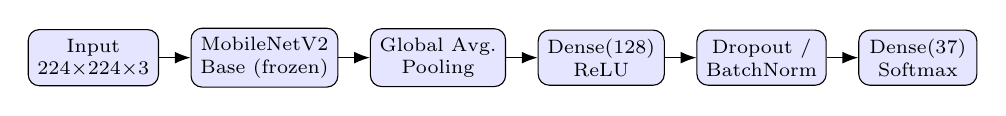
\begin{tikzpicture}[node distance=4mm]
\node[layer](a){Input\\$224{\times}224{\times}3$};
\node[layer,right=of a](b){MobileNetV2\\Base (frozen)};
\node[layer,right=of b](c){Global Avg.\\Pooling};
\node[layer,right=of c](d){Dense(128)\\ReLU};
\node[layer,right=of d](e){Dropout /\\BatchNorm};
\node[layer,right=of e](f){Dense(37)\\Softmax};
\foreach \x/\y in {a/b,b/c,c/d,d/e,e/f}
\draw[arrow](\x)--(\y);
\end{tikzpicture}
\end{center}

The Global Average Pooling output (1280 values per image) is called  the bottleneck which is  
used throughout this report. The Dense(128), optional regularization layer, and Dense(37)
softmax layer together make  the classifier head.

\section*{5. Weight Initialization}

Four initialization strategies were compared for the head's Dense(128) and Dense(37) layers,
with everything else (Adam optimizer, learning rate 0.001, 20 epochs) held fixed: Zero,
Random (small Gaussian), Xavier/Glorot, and He.

\begin{center}
\includegraphics[width=0.7\textwidth]{figures/plot1_init_train_loss.eps}
\end{center}

\textbf{Observation:} With zero initialization the training loss stays the same at about 3.61
for every epochs, which is close to $\ln(37) \approx 3.61$, the loss a model gets by making every probability equal
. Every neuron in the head starts
identical under zero initialization, so they all receive the same gradient and theres is nothing which differentiates them , and the network ends up never  learning. Random, Xavier/Glorot and He
initialization all bring the training loss down to close to zero within about 5 epochs and
stay there for the rest of training.

\begin{center}
\includegraphics[width=0.7\textwidth]{figures/plot2_init_val_acc.eps}
\end{center}

\textbf{Observation:} Validation accuracy under zero initialization stays under 2\% for the
whole run, consistent with the network never learning anything beyond a constant output.
Random, Xavier/Glorot and He all reach the 86--92\% range within the first few epochs and stay
close to each other for the rest of training, with no one method staying consistently ahead of
the other two throughout.

Test accuracy after training was 2.73\% for Zero initialization, 89.97\% for Random, 89.97\%
for Xavier/Glorot, and 89.75\% for He. Random initialization reached the highest peak
validation accuracy across epochs and was carried forward as the initialization used for
every later study in this report.

\section*{6. Regularization and Overfitting}

Four regularization options were compared, all using Random initialization for the head,
trained for 40 epochs: No Regularization, L2 Regularization (weight 0.01), Dropout (rate 0.5),
and Batch Normalization.

\begin{center}
\includegraphics[width=\textwidth]{figures/plot3_reg_accuracy.eps}
\end{center}

\textbf{Observation:}  Regularization and Batch Normalization  reaches 100\% training
accuracy while validation accuracy stays around 90--92\%, leaving a clear gap. L2
Regularization never reaches 100\% training accuracy and is the noisiest on validation.
Dropout climbs to high training accuracy more slowly than the other three.

\begin{center}
\includegraphics[width=\textwidth]{figures/plot4_reg_loss.eps}
\end{center}

\textbf{Observation:} Validation loss for No Regularization, Batch Normalization and Dropout
falls at the start  and then rises again, this is the  usual sign of overfitting. L2 Regularization keeps both
training and validation loss higher  instead.

Test accuracy was 89.67\% for No Regularization, 87.63\% for L2 Regularization, 89.29\% for
Dropout, and 89.81\% for Batch Normalization. Dropout had the highest validation accuracy and
was used in the sections below.

\section*{7. Batch Normalization}

\textbf{Numerical example.} For the mini-batch $x = [2, 4, 6, 8]$, the batch mean is
$\mu_B = 5.0$ and the batch variance is $\sigma_B^2 = 5.0$, giving
$\hat{x} \approx [-1.342,\ -0.447,\ 0.447,\ 1.342]$. With $\gamma = 1$ and $\beta = 0$, the
output equals $\hat{x}$ directly. Batch Normalization centers and scales activations within
each mini batch  and the learnable params $\gamma$ and $\beta$ let the network undo this if needed.

\begin{center}
\includegraphics[width=0.7\textwidth]{figures/plot5_bn_compare.eps}
\end{center}

\textbf{Observation:} With Batch Normalization, validation accuracy reaches its peak(best solution) faster,
by around epoch 5. Without it, accuracy increases more slowly but reaches a similar level by
epoch 10 and both stay in the 90--92\% range for the rest of training.So faster convergence .

\section*{8. Optimization Algorithms}

4 optimizers were evaluated for 25 epochs, all using Random initialization and Dropout as  0.5:
SGD (learning rate 0.01), Momentum (SGD with momentum 0.9), RMSProp (learning rate 0.001),
and Adam (learning rate 0.001).

\begin{center}
\includegraphics[width=0.7\textwidth]{figures/plot6_opt_train_loss.eps}
\end{center}

\textbf{Observation:} SGD's training loss falls but slowly, still above 0.35 by epoch 25.
Momentum, RMSProp and Adam all drop below 0.5 within a few epochs and reach close to zero.

\begin{center}
\includegraphics[width=0.7\textwidth]{figures/plot7_opt_val_acc.eps}
\end{center}

\textbf{Observation:} SGD starts at around 38\% validation accuracy and takes about 18 to 20 epochs 
reach what the other three optimizers reach within 5.

\begin{center}
\begin{tabular}{|l|c|c|c|c|}
\hline
Optimizer & Final Loss & Best Val. Accuracy & Epoch to Converge & Time (s)\\
\hline
SGD & 0.3739 & 91.03\% & 8 & 4.90\\
Momentum & 0.0529 & 92.39\% & 4 & 4.99\\
RMSProp & 0.0281 & 92.39\% & 2 & 5.65\\
Adam & 0.0327 & 92.66\% & 2 & 4.95\\
\hline
\end{tabular}
\end{center}

Adam has the highest best validation accuracy of the 4 and which were used for the
hyperparameter study, the transfer learning study, and the cross-validation configurations.

\section*{9. CNN Hyperparameter Tuning}

Three controlled sweeps were run, changing one hyperparameter at a time, starting from Random
initialization, Dropout 0.5, and Adam.

\begin{center}
\includegraphics[width=0.55\textwidth]{figures/plot8_lr_vs_valacc.eps}
\end{center}

\textbf{Observation:} A learning rate of 0.001 reached 92.66\% validation accuracy versus
91.03\% for 0.0001.

\begin{center}
\includegraphics[width=0.55\textwidth]{figures/plot9_batch_vs_valacc.eps}
\end{center}

\textbf{Observation:} Batch size 32 reached the highest accuracy at 92.66\%; both 16 and 64
gave a lower 92.12\%.

\begin{center}
\includegraphics[width=0.55\textwidth]{figures/plot10_dropout_vs_valacc.eps}
\end{center}

\textbf{Observation:} Accuracy increased with the dropout rate: 92.12\% at 0, 92.39\% at 0.25, and
92.93\% at 0.5.

The best combination, learning rate 0.001, batch size 32  and dropout rate 0.5 became
92.39\% validation accuracy and 89.64\% test accuracy when retrained.

\section*{10. Transfer Learning and Fine-Tuning}

Case A keeps the backbone frozen for 21 epochs. Case B trains frozen for 15 epochs, then
unfreezes the last 30 of MobileNetV2's 154 layers and fine-tunes for 6 more epochs at a
learning rate of $1\times10^{-5}$.

\begin{center}
\includegraphics[width=0.7\textwidth]{figures/plot11_fe_vs_ft.eps}
\end{center}

\textbf{Observation:} Both curves move the same  for the first 15 epochs. After fine-tuning
starts, the Fine-Tuning curve rises to about 92.7\% before ending at 92.1\%, while Feature
Extraction ends lower at about 90.5\%.

\begin{center}
\includegraphics[width=0.7\textwidth]{figures/plot12_ft_loss.eps}
\end{center}

\textbf{Observation:} Training loss decreases smoothly through the fine-tuning transition with
no visible spike, and validation loss stays close to flat throughout.

Test accuracy was 90.00\% for feature extraction and 89.97\% after fine-tuning, essentially
unchanged despite the higher validation accuracy.

\section*{11. K-Fold Cross-Validation}

4 setups were evaluated with 5-fold cross-validation on the frozen backbone, using
the combined training and validation data: C1 (Random initialization only), C2 (adds Dropout
0.5), C3 (adds Adam), and C4 (best combined hyperparameters from Section 9). Fine-tuning was
not included  since it would require 20 separate end-to-end training runs.

\begin{center}
\begin{tabular}{|l|c|c|c|c|c|c|c|}
\hline
Configuration & F1 & F2 & F3 & F4 & F5 & Mean & SD\\
\hline
C1: Best Init Only & 91.17 & 91.58 & 92.93 & 91.98 & 91.17 & 91.77 & 0.74\\
C2: Best Init + Best Reg & 90.76 & 91.30 & 93.07 & 92.39 & 91.85 & 91.88 & 0.90\\
C3: Best Init + Best Reg + Best Optimizer & 90.76 & 91.44 & 92.66 & 92.26 & 91.30 & 91.68 & 0.76\\
C4: Best Hyperparameters & 90.76 & 91.44 & 92.93 & 91.98 & 91.30 & 91.68 & 0.82\\
\hline
\end{tabular}
\end{center}

\begin{center}
\includegraphics[width=0.7\textwidth]{figures/plot13_cv_results.eps}
\end{center}

\textbf{Observation:} All four configurations land between 91.68\% and 91.88\% mean accuracy
with overlapping error bars. C2 had the highest mean (91.88\%, SD 0.90) and was selected for
Section 12.

\section*{12. Final Model Evaluation}

C2 was retrained on the full training and validation data (3,680 images) for 15 epochs, then
evaluated once on the untouched 3,669-image test set.

\begin{center}
\begin{tabular}{|l|c|}
\hline
Metric & Value\\
\hline
Mean CV Accuracy & 91.88\%\\
CV Standard Deviation & 0.90\\
Test Accuracy & 90.46\%\\
Precision & 90.97\%\\
Recall & 90.46\%\\
F1-score & 90.45\%\\
Training Time & 2.63 s\\
Number of Parameters & 168,741\\
\hline
\end{tabular}
\end{center}

Test accuracy is about 1.4 points lower than the mean cross-validation accuracy, expected
since the test set was never seen before this evaluation.

\begin{longtable}{|l|c|c|c|c|}
\hline
Class & Precision & Recall & F1-score & Support\\
\hline
\endfirsthead
\hline
Class & Precision & Recall & F1-score & Support\\
\hline
\endhead
Abyssinian & 0.82 & 0.91 & 0.86 & 98\\
american\_bulldog & 0.75 & 0.91 & 0.82 & 100\\
american\_pit\_bull\_terrier & 0.82 & 0.55 & 0.66 & 100\\
basset\_hound & 1.00 & 0.82 & 0.90 & 100\\
beagle & 0.84 & 0.96 & 0.90 & 100\\
Bengal & 0.80 & 0.87 & 0.83 & 100\\
Birman & 0.75 & 0.85 & 0.80 & 100\\
Bombay & 0.90 & 0.90 & 0.90 & 88\\
boxer & 0.91 & 0.85 & 0.88 & 99\\
British\_Shorthair & 0.95 & 0.77 & 0.85 & 100\\
chihuahua & 0.89 & 0.89 & 0.89 & 100\\
Egyptian\_Mau & 0.95 & 0.85 & 0.90 & 97\\
english\_cocker\_spaniel & 0.99 & 0.93 & 0.96 & 100\\
english\_setter & 0.96 & 0.97 & 0.97 & 100\\
german\_shorthaired & 0.97 & 0.97 & 0.97 & 100\\
great\_pyrenees & 0.99 & 0.99 & 0.99 & 100\\
havanese & 0.92 & 1.00 & 0.96 & 100\\
japanese\_chin & 1.00 & 0.96 & 0.98 & 100\\
keeshond & 0.96 & 1.00 & 0.98 & 99\\
leonberger & 0.99 & 0.99 & 0.99 & 100\\
Maine\_Coon & 0.87 & 0.87 & 0.87 & 100\\
miniature\_pinscher & 0.95 & 0.91 & 0.93 & 100\\
newfoundland & 0.97 & 1.00 & 0.99 & 100\\
Persian & 0.91 & 0.91 & 0.91 & 100\\
pomeranian & 0.97 & 0.91 & 0.94 & 100\\
pug & 0.97 & 0.95 & 0.96 & 100\\
Ragdoll & 0.76 & 0.76 & 0.76 & 100\\
Russian\_Blue & 0.84 & 0.85 & 0.85 & 100\\
saint\_bernard & 0.87 & 0.99 & 0.93 & 100\\
samoyed & 0.92 & 0.98 & 0.95 & 100\\
scottish\_terrier & 0.96 & 1.00 & 0.98 & 99\\
shiba\_inu & 0.94 & 0.97 & 0.96 & 100\\
Siamese & 0.97 & 0.83 & 0.89 & 100\\
Sphynx & 0.95 & 0.87 & 0.91 & 100\\
staffordshire\_bull\_terrier & 0.63 & 0.82 & 0.71 & 89\\
wheaten\_terrier & 1.00 & 0.92 & 0.96 & 100\\
yorkshire\_terrier & 0.99 & 0.99 & 0.99 & 100\\
\hline
Macro Avg & 0.91 & 0.90 & 0.90 & 3669\\
Weighted Avg & 0.91 & 0.90 & 0.90 & 3669\\
\hline
\end{longtable}

\begin{center}
\includegraphics[width=0.95\textwidth]{figures/plot14_confusion_matrix.eps}
\end{center}

\textbf{Observation:} Most classes reach a clean diagonal, several with an F1-score near 0.99.
The biggest confusion in this matrix is between american\_pit\_bull\_terrier and
staffordshire\_bull\_terrier, matching their low recall and precision above. Smaller confusions
appear among visually similar cat breeds.

\begin{center}
\includegraphics[width=\textwidth]{figures/plot15_misclassified.eps}
\end{center}

\textbf{Observation:} The misclassified examples follow the same pattern: look-alike breed
pairs such as boxer/american\_bulldog, Abyssinian/Russian\_Blue, and Maine\_Coon/Bengal.

\section*{13. Overall Results}

\begin{center}
\begin{tabular}{|l|c|c|c|}
\hline
Configuration & Val. Accuracy (\%) & Test Accuracy (\%) & Training Time (s)\\
\hline
Baseline & 92.93 & 90.43 & 3.48\\
Best Initialization & 92.12 & 89.97 & 3.82\\
Best Regularization & 93.21 & 89.29 & 7.63\\
Best Optimizer & 92.66 & 90.19 & 4.95\\
Best Hyperparameters & 92.39 & 89.64 & 4.28\\
Fine-Tuned Model & 92.66 & 89.97 & 46.00\\
\hline
\end{tabular}
\end{center}

Baseline uses default settings with no tuning; the middle four rows are the single best model
from each section; Fine-Tuned Model is the Case B model from Section 10. Only Section 11's
four configurations went through cross-validation.

Baseline had the highest test accuracy of the six rows, at 90.43\%, though all six are within
about two points of each other. The Fine-Tuned Model took by far the longest to train, since it
is the only row that updates the backbone directly on images instead of a cached-feature head.

\section*{14. Required Inference for Plots}

Each plot in this report is followed directly by an observation describing what the plot
shows, the trend visible in it, and a possible reason for that trend, rather than being
collected separately in this section.

\section*{15. Discussion Questions}

\begin{enumerate}
\item \textbf{What is the difference between model parameters and hyperparameters?}
Parameters are learned from data during training, such as the weights and biases in the Dense
layers. Hyperparameters are set before training, such as learning rate, batch size, dropout
rate and optimizer choice.These are for us to tune 

\item \textbf{Why is weight initialization important?}
The starting weights affect how gradients flow early in training. A poor starting point can
slow convergence or, as with zero initialization, stop learning altogether.

\item \textbf{Why can zero initialization be problematic for neural networks?}
Every neuron starts identical and receives the same gradient, so none of them differentiate.
This kept training loss flat near $\ln(37)$ in Section 5.

\item \textbf{Compare Xavier and He initialization.}
Xavier/Glorot sets variance based on fan-in and fan-out and suits sigmoid/tanh. He uses only
fan-in with a larger variance and suits ReLU. Both performed almost identically here, 89.97\%
versus 89.75\% test accuracy.

\item \textbf{How can training and validation curves be used to identify overfitting?}
Overfitting shows as training accuracy or loss continuing to improve while validation accuracy
plateaus or validation loss rises, as seen in Section 6.

\item \textbf{How does Dropout reduce overfitting?}
It randomly deactivates neurons during training so the network cannot rely too heavily on any
one of them, which slows memorization of the training set.

\item \textbf{What is the purpose of Batch Normalization?}
It normalizes a layer's activations using the current mini-batch's mean and variance, making
training more stable and often faster to converge.

\item \textbf{Explain the numerical Batch Normalization example.}
For $x = [2, 4, 6, 8]$, the mean is 5 and the variance is 5, giving normalized values
$[-1.342, -0.447, 0.447, 1.342]$.

\item \textbf{What are the roles of $\gamma$ and $\beta$?}
They rescale and shift the normalized activations, letting the network recover a different
scale or the original values if that works better for a layer.

\item \textbf{Compare SGD, Momentum, RMSProp and Adam.}
SGD takes fixed-size steps and was the slowest to converge here. Momentum adds a running
average of past gradients. RMSProp scales the learning rate by recent squared gradients. Adam
combines both and reached the best accuracy, 92.66\%.

\item \textbf{What happens when the learning rate is too large?}
Training loss can oscillate or diverge instead of decreasing steadily.

\item \textbf{What happens when the learning rate is too small?}
Training becomes very slow; 0.0001 reached only 91.03\% here versus 92.66\% for 0.001.

\item \textbf{What is the effect of increasing batch size?}
A larger batch gives a more stable gradient estimate but fewer updates per epoch. Batch size
32 worked best in this experiment.

\item \textbf{Explain stride and padding.}
Stride is how far the kernel moves between positions. Padding adds border pixels so the output
size can be controlled and edges can be covered.

\item \textbf{Why is MobileNetV2 computationally efficient?}
It uses depthwise separable convolutions instead of standard convolutions, cutting the number
of parameters and multiplications sharply.

\item \textbf{What is depthwise separable convolution?}
A depthwise convolution applies one filter per channel, followed by a $1\times1$ pointwise
convolution that mixes the channels.

\item \textbf{What is transfer learning?}
Reusing a model already trained on a large dataset, usually ImageNet, as the starting point
for a new task instead of training from scratch.

\item \textbf{Differentiate feature extraction and fine-tuning.}
Feature extraction keeps the backbone frozen and trains only the head. Fine-tuning also
unfreezes some backbone layers and trains them at a low learning rate.

\item \textbf{Why is a smaller learning rate generally used during fine-tuning?}
A large learning rate risks damaging the pretrained weights before they can adapt gently to
the new data.

\item \textbf{Why is K-Fold Cross-Validation useful for hyperparameter selection?}
It averages performance over several data splits, giving a more reliable estimate and showing
how much the split itself matters.

\item \textbf{Why must the test set remain untouched during tuning?}
Using it during tuning would make later test accuracy an unfair estimate of performance on
genuinely unseen data.

\item \textbf{Why should mean and standard deviation both be reported?}
The mean alone does not show consistency across splits; two configurations can share a mean
but differ in standard deviation.

\item \textbf{Is the highest validation accuracy always sufficient to select a model?}
No. In Section 13, Baseline had a lower validation accuracy than several rows but the highest
test accuracy, so other factors matter too.
\end{enumerate}

\section*{16. Additional Exercise}

Two new hyperparameter combinations were tested with 5-fold cross-validation and compared
against C2, both keeping the backbone frozen for the same reason as Section 11.

\begin{center}
\begin{tabular}{|l|c|c|}
\hline
Configuration & Mean Accuracy (\%) & SD\\
\hline
C2: Best Init + Best Reg (selected in Section 11) & 91.88 & 0.90\\
New Combo 1 (LR = 0.0005, Dropout = 0.3, Batch = 48) & 91.66 & 0.81\\
New Combo 2 (LR = 0.0003, Dropout = 0.6, Batch = 24) & 91.55 & 0.73\\
\hline
\end{tabular}
\end{center}

Neither new combination beat C2's mean accuracy, though both had a slightly lower standard
deviation. C2 remains the preferred configuration.

\section*{17. Expected Outcome}

Initialization, regularization, optimizer choice and hyperparameters all affected performance,
though most differences were small next to the run-to-run variation seen across
cross-validation folds. Zero initialization was the one setting that caused outright failure.
Fine-tuning improved validation accuracy but not test accuracy. The final selected
configuration reached 90.46\% test accuracy, 90.97\% precision, 90.46\% recall and 90.45\%
F1-score.

\section*{18. References}

\begin{enumerate}
\item Ian Goodfellow, Yoshua Bengio and Aaron Courville, \emph{Deep Learning}, MIT Press, 2016.
\item Sergey Ioffe and Christian Szegedy, ``Batch Normalization: Accelerating Deep Network
Training by Reducing Internal Covariate Shift,'' ICML, 2015.
\item Mark Sandler, Andrew Howard, Menglong Zhu, Andrey Zhmoginov and Liang-Chieh Chen,
``MobileNetV2: Inverted Residuals and Linear Bottlenecks,'' CVPR, 2018.
\item Omkar M. Parkhi, Andrea Vedaldi, Andrew Zisserman and C. V. Jawahar, ``Cats and Dogs,''
IEEE Conference on Computer Vision and Pattern Recognition, 2012.
\item TensorFlow Documentation: \url{https://www.tensorflow.org}
\item Keras Documentation: \url{https://keras.io}
\end{enumerate}

\end{document}
